% La conclusión debe contener los principales aspectos y contribuciones para finalizar el trabajo presentado. Se debe presentar lo que se esperaba del trabajo a través de los objetivos introducidos inicialmente y mostrar lo que se logró. No se debe insertar un nuevo asunto en la conclusión. Aquí el autor presentará las propias impresiones sobre el trabajo efectuado. Es importante también que se identifiquen limitaciones y problemas que surgieron durante el desarrollo del trabajo y cuáles las consecuencias del mismo.

% Los trabajos futuros deben contener oportunidades de expansión del trabajo presentado, así como nuevos proyectos que pudieron ser vislumbrados a partir del desarrollo del trabajo.

\chapter{Conclusiones y Trabajo Futuro}
\label{ch:Conclusiones y Trabajo Futuro}

\begin{quote}
  {\bf\textsc{Resumen:}} Este capítulo recoge los principales aspectos y contribuciones obtenidos para la integración de Información Geográfica en la Web Semántica. De igual manera, comprobaremos el cumplimiento de los objetivos que introducimos inicialmente en el \texttt{capítulo 1}. Asimismo, se comentarán posibles propuestas de mejora de cara a posibles iteraciones del proyecto, además de comentar otras posibles aplicaciones relacionadas, que caen fuera del ámbito de este trabajo.
\end{quote}




\section{Conclusiones}

En este TFM se ha profundizado en el uso de la Web Semántica Geoespacial, en concreto en la posibilidad de integrar Información Geográfica en la Web Semántica mediante el uso de herramientas específicas, a través de la creación de la ontología GEOARES. Se han estudiado algunas de las tecnologías que se pueden utilizar para representar e integrar Información Geográfica, como los lenguajes de ontologías (RDF, OWL) y de consultas (SPARQL y GeoSPARQL). Se han valorado las herramientas de la Web Semántica para permitir crear la ontología, como GraphDB y Protegé, esta última no ha permitido incluir el \textit{plugin} de GeoSPARQL, no obstante, la alternativa encontrada, GraphDB, ha permitido solventar los problemas ocasionados con Protegé. \\

Así, se ha desarrollado una prueba de concepto trabajando con información geoespacial, concretamente con archivos en formato \textit{Shapefile} de la provincia de Granada, en particular de mi pueblo, Ogíjares, y centrándonos en la información geoespacial obtenida de edificaciones, puntos de cota y curvas de nivel, para su integración en la ontología y su posterior visualización en un mapa a través de R. Dentro de todas las posibilidades de análisis que ofrece la Web Semántica, se ha prestado especial atención a la relacionada con Información Geográfica, en donde, gracias a los estándares definidos, es decir, las funciones usadas en GeoSPARQL, las cuales son las mismas que OGC ha definido en su estándar para el tratamiento de datos SIG, es posible combinar dos ámbitos que previamente parecían ser independientes el uno respecto del otro. Entonces, se han utilizado tecnologías tanto de la Web Semática como de los SIG que nos allanan el camino para ambas áreas, permitiendo la heterogeneidad e interoperabilidad de los datos geográficos gracias a la capa semántica que estos presentan.\\


%Se ha apreciado, que las funciones usadas en el GeoSPARQL son las mismas que OGC ha definido en su estándar. Con esto acabamos de comprobar como ha sido posible unir dos ámbitos que previamente parecían ser independientes el uno respecto del otro.
A la vista de los resultados obtenidos, considero que haber realizado esta prueba de concepto me ha abierto nuevos puntos de vista hacia otra perspectiva de la Web. Parte de mi contribucción ha sido enseñar las herramientas que facilitan el trabajo para la puesta en marcha de una ontología. Por tanto, mediante el desarrollo de este TFM, valoro que se han conseguido los objetivos señalados en la \texttt{subsección \ref{ch:objetivos}} del \texttt{capítulo \ref{ch:introduccion}}, en concreto:


\begin{enumerate}
	
	\item Se ha mostrado mediante la utilización de la Web Semántica Geoespacial, cómo los estándares que se usan en el lenguaje de consulta geoespacial corresponden a los mismos definidos por el organismo OGC para los datos geográficos (ver \texttt{capítulo \ref{ch:capitulo4}}).
	%\item \textbf{Comprender la relación existente entre los Sistemas de Información Geográfica y la Web Semántica}, a priori dos áreas completamente diferentes.
	
	\item Se han definido dos fuentes principales de información con las que obtener datos públicos geográficos de buena calidad y se han usado los datos de una de ellas, en concreto los del Instituto de Estadística y Cartografía de Andalucía (ver \texttt{sección \ref{ch:capitulo5-datos}}).
	
	%\item \textbf{Hacer uso de fuentes de información geoespacial}, con las que obtener datos públicos geográficos de buena calidad.
	
	\item Se han considerado herramientas de la Web Semántica de gran alcance para representar e integrar Información Geográfica, entre las que destacamos Protegé y GraphDB (ver \texttt{capítulo \ref{ch:capitulo5}}).
	%\item \textbf{Localizar diversas herramientas de la Web Semántica} que se puedan utilizar para representar e integrar Información Geográfica.
	
	\item Se ha mostrado mediante Protegé cómo es posible agregar conocimiento de dominio geoespacial sobre la estructura de los datos de manera sencilla (ver \texttt{sección \ref{ch:crear}}).
	%\item Aprender a \textbf{agregar conocimiento de dominio geoespacial sobre la estructura de los datos} mediante el empleo de herramientas de la Web Semántica como Protegé.
	
	\item Se ha mostrado mediante Protegé cómo es posible poblar una ontología de manera eficaz haciendo uso de diversas reglas (ver \texttt{sección \ref{ch:poblar}}).
	%\item \textbf{Aprender a crear ontologías y poblarlas}  mediante información geográfica existente.
	
	\item Se ha realizado un estudio acerca de las carencias o mejoras que supone usar Protegé (ver \texttt{Apéndice \ref{ch:ApendiceB}}).
	%\item Apreciar las carencias o mejoras que supone usar \textbf{Protegé frente a otro tipo de herramientas}.
	
	\item Se han mostrado la estructura de los datos geoespaciales y sus especificaciones para realizar consultas con el lenguaje GeoSPARQL (ver \texttt{sección \ref{ch:capitulo4-geosparql}} y \texttt{sección \ref{ch:consultas}}).
	%\item Conocer cuál es la \textbf{estructura de los datos geoespaciales y sus especificaciones para realizar consultas con el lenguaje GeoSPARQL}.
	
	\item Se ha aprendido a crear un mapa Web en R mediante el uso de la biblioteca \textit{Leaflet} y el framework \textit{Shiny} para ubicar información geoespacial en un mapa (ver \texttt{sección \ref{ch:visualizacion}}).
	%\item Aprender a \textbf{ubicar información geoespacial en un mapa mediante el uso de la biblioteca Leaflet}.
	
	\item Se ha mostrado, mediante ejemplos, formas de trabajo sobre la Web Semántica Geoespacial (ver \texttt{capítulo \ref{ch:capitulo5}}).
	%\item Mostrar algunos \textbf{métodos de trabajo}, estrechamente adaptados al tratamiento de Información Geográfica en la Web Semántica.
	
	\item Se ha prestado especial atención a desarrollar un trabajo autocontenido, tratando que sea accesible a cualquier persona con un perfil tecnológico básico que esté interesado en el tema.
	
	%\item \textbf{Aportaciones a la comunidad o al lector}, para que el proyecto sirva como puerta de acceso al mundo de la Web Semántica y en particular, al de la Web Semántica Geoespacial, y facilite el acceso a parte de los conocimientos actuales disponibles.
	
	\item He adquirido experiencia y conocimientos en un tema nuevo para mí, la Web Semántica, y ampliado otros como el caso de los Sistemas de Información Geográfica.
	%\item \textbf{Aportaciones hacia mi persona} en la puesta en práctica y adquisición de conocimiento de los anteriores puntos.
	%\item \textbf{Aportaciones hacia mi persona} en la adquisición de conocimientos de la Web Semántica, creación de ontologías, manejo de herramientas semánticas como Protegé y aprendizaje para la creación de un mapa interactivo mediante la librería Shiny de R.	
	
	

	
\end{enumerate}



%La WS es aún una visión, un proyecto de futuro muy ambicioso, que permitirá, con ayuda de la Inteligencia Artificial, realizar un sinfín de operaciones en la Web, mucho más amplias que las ofertadas hoy en día. El tener toda la información etiquetada sintáctica y semánticamente facilitará la implementación eficaz de los llamados agentes inteligentes, capaces de ofrecer información Web pertinente, en función de los intereses y circunstancias personales de cada usuario (personalización máxima).



%Esta situación imaginaria tiene ya su base real, materializada en los proyectos piloto realizados y en los grandes avances logrados para su creación en cuanto a estándares e infraestructura. Las principales empresas, como IBM, Microsoft, etc. participan activamente en su desarrollo, así como la comunidad investigadora, especialmente la universitaria. Por supuesto, el proyecto no hubiera sido posible sin el apoyo e impulso de la W3C, que junto con el sitio oficial www.semanticweb.org, se encarga de ofrecer toda la información disponible sobre los progresos en este ámbito. El interés por la WS se refleja en la celebración anual del Congreso internacional de la WWW, que en 2009 ha tenido lugar en la Universidad Politécnica de Madrid. También queda patente con la publicación de la revista Journal of Web Semantics.

%En el terreno de las bibliotecas, la WS podrá ser decisiva de cara a la construcción de una Biblioteca Digital Universal, donde todo sea accesible de forma rápida y precisa, se encuentre donde se encuentre. Por supuesto, aún queda mucho camino por recorrer y la transición de la Web actual a la WS puede implicar un coste altísimo (en tiempo, dinero y esfuerzo), ya que no sólo se trata de estructurar la información web venidera, sino también la ya existente, labor que se prevé irrealizable.

\section{Proyectos relacionados}

Dentro de los proyectos relacionados con la Web Semántica y los SIG, destacan los documentados en el libro \textit{\textbf{Geospatial Semantic Web}} de \textit{Chuanrong Zhang}, \textit{Tian Zhao} y \textit{Weidong Li}. Este libro cubre temas clave relacionados con la Web Semántica Geoespacial; ontología geoespacial para la interoperabilidad semántica; creación, intercambio e integración de ontologías; desafíos de la Web Semántica Geoespacial; desarrollo de aplicaciones Web Semánticas Geoespaciales, entre otros. Asimismo, se describen tecnologías, como WFS, WMS, RDF, OWL y GeoSPARQL, y muestra cómo usar las tecnologías de la Web Semántica Geoespacial para resolver problemas prácticos del mundo real, como los datos espaciales \cite{libro-gis}. \\

También son remarcables los trabajos siguientes: ``La Web semántica y las tecnologías del lenguaje humano'' en \cite{researchgate}, ``Geography 2.0—A mash-up perspective'' \cite{gml} y ``Data Models and Query Languages for Linked Geospatial Data'' en \cite{wkt-database}; en donde se cubren las áreas de la Web Semántica, SIG y la combinación de ambas, entre otros.\\

Por otro lado, destacar un proyecto de la Universidad de Almería \textbf{XOSM}, \textit{XQuery for OpenStreetMap} (\url{http://xosm.ual.es/XOSM/query.php}), que hace uso de la Información Geográfica Voluntaria mediante OpenStreetMap (OSM) para ofrecer datos de mapas urbanos y rurales. XOSM es una herramienta para el procesamiento de consultas geoespaciales en OSM equipada con un lenguaje de consulta basado en un conjunto de operadores definidos para OSM implementados como una biblioteca del lenguaje de consulta \textit{XML XQuery}. Esta biblioteca proporciona un repertorio de funciones espaciales que actúan sobre la representación XML de una capa OSM y permite la definición de consultas que combinan capas OSM y capas creadas a partir de recursos de datos abiertos vinculados (KML, GeoJSON, CSV y RDF). \\

En la figura \ref{fig:1-6} se puede observar la página de inicio de esta herramienta, en donde, explica en que consiste. 


% COMENTAR FIGURAS


%LOs datos se crean con KML (xosm.ual.es)

\begin{figure}[H]
	\centering
	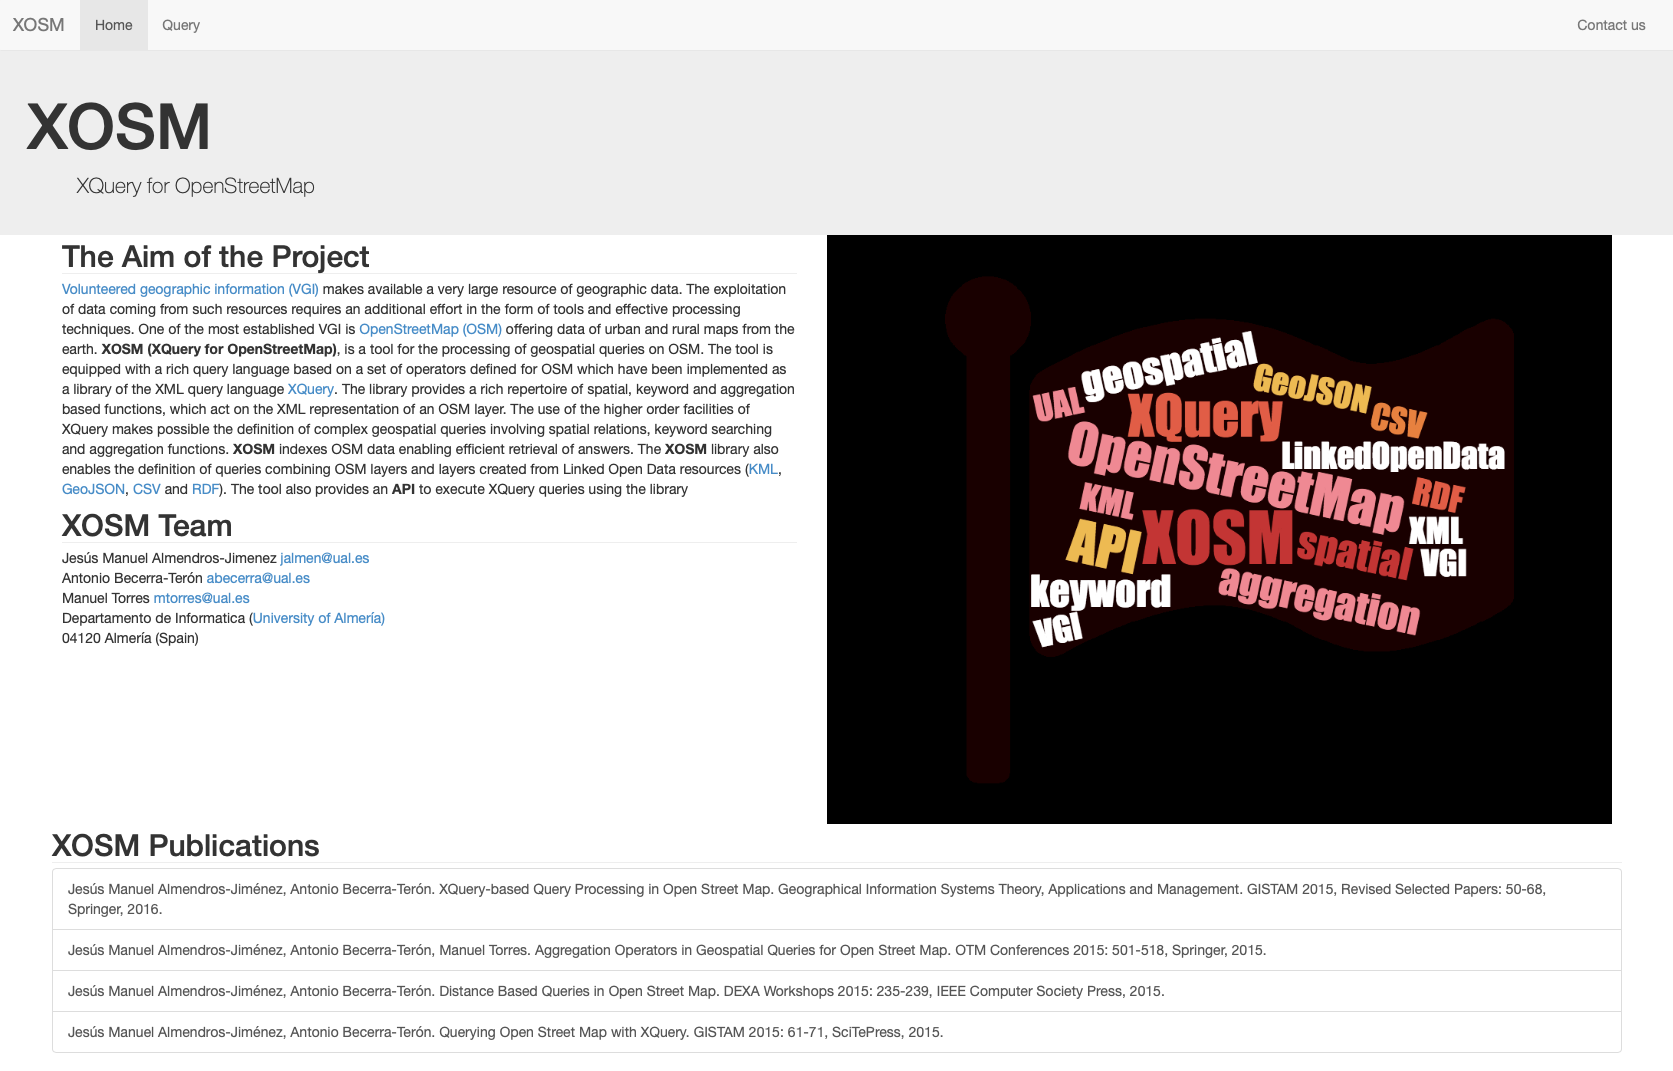
\includegraphics[width=1\linewidth]{imagenes/capitulo6/1}
	\caption{Página de inicio de XOSM}
	\label{fig:1-6}
\end{figure}

Por otro lado, las figuras \ref{fig:2-6} y \ref{fig:3-6} nos muestran un ejemplo del funcionamiento de XOSM en donde se representan en un mapa las calles de Londres que cruzan la calle \textit{Haymarket} y tocan \textit{Trafalgar Square}.

\begin{figure}[H]
	\centering
	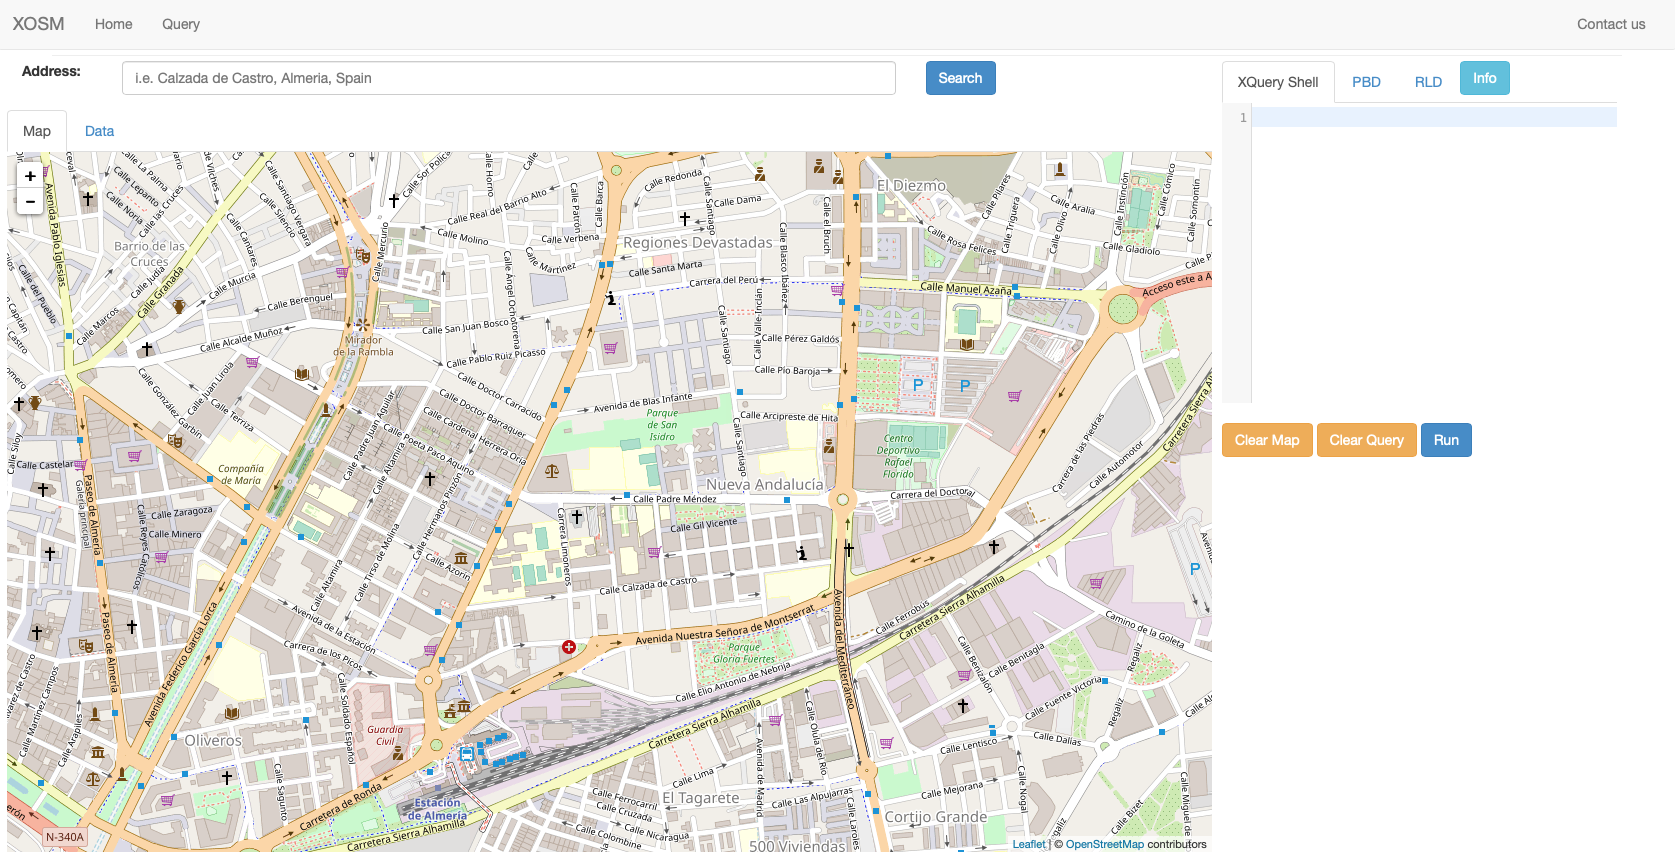
\includegraphics[width=1\linewidth]{imagenes/capitulo6/2}
	\caption{Hacer consulta en XOSM}
	\label{fig:2-6}
\end{figure}

\begin{figure}[H]
	\centering
	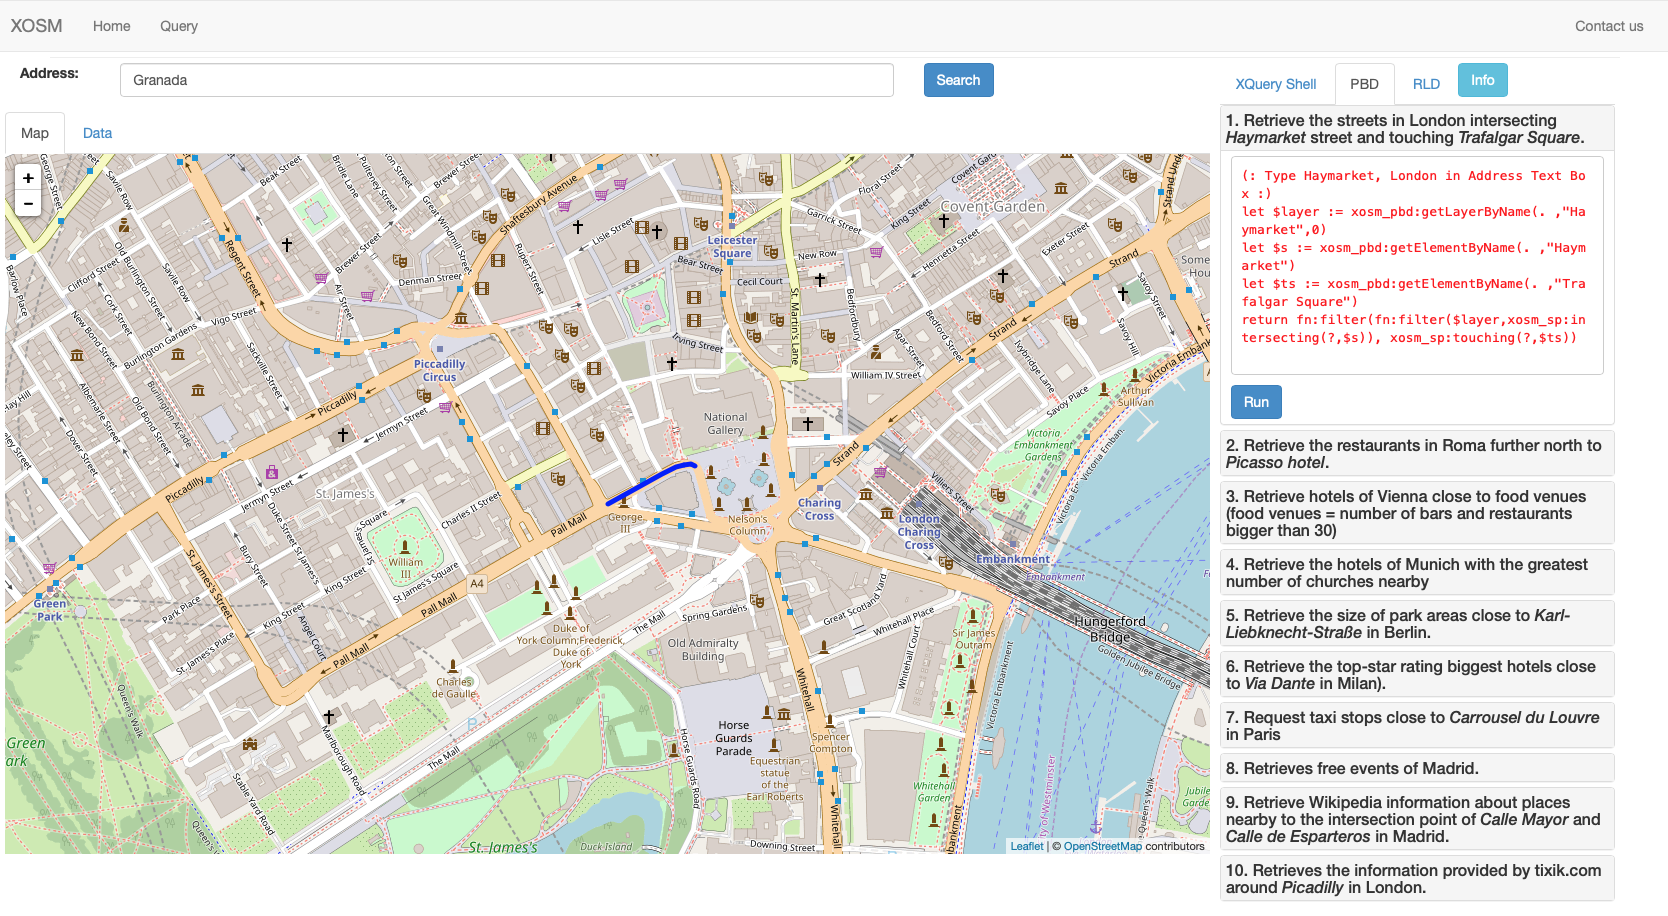
\includegraphics[width=1\linewidth]{imagenes/capitulo6/3}
	\caption{Salida de una consulta de ejemplo en XOSM}
	\label{fig:3-6}
\end{figure}


Y cómo se observa, este TFM se mantiene en la línea de estos proyectos.

\section{Trabajo futuro}

Durante la realización de este TFM se han encontrado o han podido surgir temas, ejemplos o aplicaciones bastantes relacionados pero que no se han estudiado en el mismo, por este motivo, comentaremos algunos aspectos a profundizar en el futuro:

\begin{enumerate}
	
	\item Crear una plataforma parecida a la mostrada en las figuras \ref{2-6} y \ref{fig:3-6}, en donde, a partir de la salida de la consulta que se haga, obtener el GID ubicado automáticamente en el mapa, es decir, integrar en una herramienta la prueba de concepto realizada.
	
	\item Generar otro ejemplo con la misma Información Geográfica pero obtenida de otra parte, para comprobar cómo la Web Semántica, gracias a su estructura, permite la heterogeneidad.
	
	%\item Generar modelos para obtener la temperatura de una superficie a partir de la altitud y la localización del territorio.
	%\item Realizar un estudio con la función $terrain$ de R para la rugosidad del terreno, ya que dicha función no sólo permite obtener la pendiente y la orientación, sino otras variables cartográficas.
	%\item Ampliar el paquete desarrollado para facilitar este tipo de análisis, así como, aumentar el volumen de datos cargados en la misma, centrándonos en los MDT de España.
\end{enumerate}

Adicionalmente, considero que este tema y el enfoque que le he dado puede tener interés para el público en general por lo que valoro la posibilidad de darle más difusión al trabajo.



